% This is "sig-alternate.tex" V2.1 April 2013
% This file should be compiled with V2.5 of "sig-alternate.cls" May 2012
%
% This example file demonstrates the use of the 'sig-alternate.cls'
% V2.5 LaTeX2e document class file. It is for those submitting
% articles to ACM Conference Proceedings WHO DO NOT WISH TO
% STRICTLY ADHERE TO THE SIGS (PUBS-BOARD-ENDORSED) STYLE.
% The 'sig-alternate.cls' file will produce a similar-looking,
% albeit, 'tighter' paper resulting in, invariably, fewer pages.
%
% ----------------------------------------------------------------------------------------------------------------
% This .tex file (and associated .cls V2.5) produces:
%       1) The Permission Statement
%       2) The Conference (location) Info information
%       3) The Copyright Line with ACM data
%       4) NO page numbers
%
% as against the acm_proc_article-sp.cls file which
% DOES NOT produce 1) thru' 3) above.
%
% Using 'sig-alternate.cls' you have control, however, from within
% the source .tex file, over both the CopyrightYear
% (defaulted to 200X) and the ACM Copyright Data
% (defaulted to X-XXXXX-XX-X/XX/XX).
% e.g.
% \CopyrightYear{2007} will cause 2007 to appear in the copyright line.
% \crdata{0-12345-67-8/90/12} will cause 0-12345-67-8/90/12 to appear in the copyright line.
%
% ---------------------------------------------------------------------------------------------------------------
% This .tex source is an example which *does* use
% the .bib file (from which the .bbl file % is produced).
% REMEMBER HOWEVER: After having produced the .bbl file,
% and prior to final submission, you *NEED* to 'insert'
% your .bbl file into your source .tex file so as to provide
% ONE 'self-contained' source file.
%
% ================= IF YOU HAVE QUESTIONS =======================
% Questions regarding the SIGS styles, SIGS policies and
% procedures, Conferences etc. should be sent to
% Adrienne Griscti (griscti@acm.org)
%
% Technical questions _only_ to
% Gerald Murray (murray@hq.acm.org)
% ===============================================================
%
% For tracking purposes - this is V2.0 - May 2012

\documentclass{sig-alternate-05-2015}


\begin{document}
\[% Copyright
%\setcopyright{acmcopyright}
%\setcopyright{acmlicensed}
%\setcopyright{rightsretained}
%\setcopyright{usgov}
%\setcopyright{usgovmixed}
%\setcopyright{cagov}
%\setcopyright{cagovmixed}


% DOI
%\doi{10.475/123_4}

% ISBN
%\isbn{123-4567-24-567/08/06}

%Conference
%\conferenceinfo{PLDI '13}{June 16--19, 2013, Seattle, WA, USA}

%\acmPrice{\$15.00}

%
% --- Author Metadata here ---
%\conferenceinfo{WOODSTOCK}{'97 El Paso, Texas USA}
%\CopyrightYear{2007} % Allows default copyright year (20XX) to be over-ridden - IF NEED BE.
%\crdata{0-12345-67-8/90/01}  % Allows default copyright data (0-89791-88-6/97/05) to be over-ridden - IF NEED BE.
% --- End of Author Metadata ---

%\title{Alternate {\ttlit ACM} SIG Proceedings Paper in LaTeX
%Format\titlenote{(Produces the permission block, and
%copyright information). For use with
%SIG-ALTERNATE.CLS. Supported by ACM.}}
%\subtitle{[Extended Abstract]
%\titlenote{A full version of this paper is available as
%\textit{Author's Guide to Preparing ACM SIG Proceedings Using
%\LaTeX$2_\epsilon$\ and BibTeX} at
%\texttt{www.acm.org/eaddress.htm}}}
\title{Robot Navigation Path Teaching: A Comparative Study of Trajectory Demonstrations and Keyframe Demonstrations}
%
% You need the command \numberofauthors to handle the 'placement
% and alignment' of the authors beneath the title.
%
% For aesthetic reasons, we recommend 'three authors at a time'
% i.e. three 'name/affiliation blocks' be placed beneath the title.
%
% NOTE: You are NOT restricted in how many 'rows' of
% "name/affiliations" may appear. We just ask that you restrict
% the number of 'columns' to three.
%
% Because of the available 'opening page real-estate'
% we ask you to refrain from putting more than six authors
% (two rows with three columns) beneath the article title.
% More than six makes the first-page appear very cluttered indeed.
%
% Use the \alignauthor commands to handle the names
% and affiliations for an 'aesthetic maximum' of six authors.
% Add names, affiliations, addresses for
% the seventh etc. author(s) as the argument for the
% \additionalauthors command.
% These 'additional authors' will be output/set for you
% without further effort on your part as the last section in
% the body of your article BEFORE References or any Appendices.

\numberofauthors{2} %  in this sample file, there are a *total*
% of EIGHT authors. SIX appear on the 'first-page' (for formatting
% reasons) and the remaining two appear in the \additionalauthors section.
%
\author{
% You can go ahead and credit any number of authors here,
% e.g. one 'row of three' or two rows (consisting of one row of three
% and a second row of one, two or three).
%
% The command \alignauthor (no curly braces needed) should
% precede each author name, affiliation/snail-mail address and
% e-mail address. Additionally, tag each line of
% affiliation/address with \affaddr, and tag the
% e-mail address with \email.
%
% 1st. author
\alignauthor
Miao Qi\\
       \email{qimiao@utexas.edu}
% 2nd. author
\alignauthor
Chunheng Luo\\
       \email{chunheng.luo@utexas.edu}
%% 3rd. author
%\alignauthor Lars Th{\o}rv{\"a}ld\titlenote{This author is the
%one who did all the really hard work.}\\
%       \affaddr{The Th{\o}rv{\"a}ld Group}\\
%       \affaddr{1 Th{\o}rv{\"a}ld Circle}\\
%       \affaddr{Hekla, Iceland}\\
%       \email{larst@affiliation.org}
%\and  % use '\and' if you need 'another row' of author names
%% 4th. author
%\alignauthor Lawrence P. Leipuner\\
%       \affaddr{Brookhaven Laboratories}\\
%       \affaddr{Brookhaven National Lab}\\
%       \affaddr{P.O. Box 5000}\\
%       \email{lleipuner@researchlabs.org}
%% 5th. author
%\alignauthor Sean Fogarty\\
%       \affaddr{NASA Ames Research Center}\\
%       \affaddr{Moffett Field}\\
%       \affaddr{California 94035}\\
%       \email{fogartys@amesres.org}
%% 6th. author
%\alignauthor Charles Palmer\\
%       \affaddr{Palmer Research Laboratories}\\
%       \affaddr{8600 Datapoint Drive}\\
%       \affaddr{San Antonio, Texas 78229}\\
%       \email{cpalmer@prl.com}
}
% There's nothing stopping you putting the seventh, eighth, etc.
% author on the opening page (as the 'third row') but we ask,
% for aesthetic reasons that you place these 'additional authors'
% in the \additional authors block, viz.
%\additionalauthors{Additional authors: John Smith (The Th{\o}rv{\"a}ld Group,
%email: {\texttt{jsmith@affiliation.org}}) and Julius P.~Kumquat
%(The Kumquat Consortium, email: {\texttt{jpkumquat@consortium.net}}).}
%\date{30 July 1999}
% Just remember to make sure that the TOTAL number of authors
% is the number that will appear on the first page PLUS the
% number that will appear in the \additionalauthors section.

\maketitle
\begin{abstract}
%This paper provides a sample of a \LaTeX\ document which conforms,
%somewhat loosely, to the formatting guidelines for
%ACM SIG Proceedings. It is an {\em alternate} style which produces
%a {\em tighter-looking} paper and was designed in response to
%concerns expressed, by authors, over page-budgets.
%It complements the document \textit{Author's (Alternate) Guide to
%Preparing ACM SIG Proceedings Using \LaTeX$2_\epsilon$\ and Bib\TeX}.
%This source file has been written with the intention of being
%compiled under \LaTeX$2_\epsilon$\ and BibTeX.
%
%The developers have tried to include every imaginable sort
%of ``bells and whistles", such as a subtitle, footnotes on
%title, subtitle and authors, as well as in the text, and
%every optional component (e.g. Acknowledgments, Additional
%Authors, Appendices), not to mention examples of
%equations, theorems, tables and figures.
%
%To make best use of this sample document, run it through \LaTeX\
%and BibTeX, and compare this source code with the printed
%output produced by the dvi file. A compiled PDF version
%is available on the web page to help you with the
%`look and feel'.
Policy learning enables a robot to select an action based on the current world state. It is the core of many modern robotic applications. Learning from Demonstration (LfD) is the policy learning approach within which a policy is learned from examples, or demonstrations, given by a teacher. In this paper, we explore different demonstration methods in robot Learning from Demonstration. Specifically, two demonstration methods, TD and KD, are compared in terms of their effectiveness and the human teacher's task load. Algorithms are implemented based on our mobile robotic platform, Sphero SPRK, and experiments are designed and conducted to do the comparison using both quantitative measures and survey results. Our experimental results show that, in general, while TD requires less task load from the human teacher, KD is more effective in terms of the robot's performance of reproducing the demonstrated navigation path. Our experiments also reveal that human teacher's strategies have a considerable effect on the effectiveness of teaching: Different human teachers tend to use different teaching strategies, and they usually deliberately adjust their strategies between demonstrations attempting to improve the robot's learning performance. 
\end{abstract}


%
% The code below should be generated by the tool at
% http://dl.acm.org/ccs.cfm
% Please copy and paste the code instead of the example below. 
%
%\begin{CCSXML}
%<ccs2012>
% <concept>
%  <concept_id>10010520.10010553.10010562</concept_id>
%  <concept_desc>Computer systems organization~Embedded systems</concept_desc>
%  <concept_significance>500</concept_significance>
% </concept>
% <concept>
%  <concept_id>10010520.10010575.10010755</concept_id>
%  <concept_desc>Computer systems organization~Redundancy</concept_desc>
%  <concept_significance>300</concept_significance>
% </concept>
% <concept>
%  <concept_id>10010520.10010553.10010554</concept_id>
%  <concept_desc>Computer systems organization~Robotics</concept_desc>
%  <concept_significance>100</concept_significance>
% </concept>
% <concept>
%  <concept_id>10003033.10003083.10003095</concept_id>
%  <concept_desc>Networks~Network reliability</concept_desc>
%  <concept_significance>100</concept_significance>
% </concept>
%</ccs2012>  
%\end{CCSXML}

%\ccsdesc[500]{Computer systems organization~Embedded systems}
%\ccsdesc[300]{Computer systems organization~Redundancy}
%\ccsdesc{Computer systems organization~Robotics}
%\ccsdesc[100]{Networks~Network reliability}


%
% End generated code
%

%
%  Use this command to print the description
%
\printccsdesc

% We no longer use \terms command
%\terms{Theory}

\keywords{Robotics; Learning from Demonstration}

\section{Introduction}
Policy learning enables a robot to select an action based on the current world state. It is the core of many modern robotic applications. Learning from Demonstration (LfD) is the policy learning approach within which a policy is learned from examples, or demonstrations, given by a teacher. LfD algorithms utilizes the demonstrations to derive a policy that reproduces the demonstrated behavior. [3] In this paper, we focus on the ``path teaching'' scenario where a human teacher remotely guides the robot to navigate through a specific path. The scenario is common in everyday practical applications, e.g., training robotic guides or auto-navigating cleaning robots used in museums, shopping malls, hospitals, homes, etc. 


In LfD, the approaches for providing demonstration data can be categorized into two types, i.e., teleoperation and shadowing. [3] In teleoperation, the teacher operates the robot learner platform and the robot's sensors keep record of the execution. In shadowing, the robot learner records the execution using sensors while attempting to mimic the teacher's motion as the teacher executes the task. This paper focuses on a specific scenario of teleoperation, where the teacher remotely operates the robot learner through speech dialog. Such an approach has the advantage that it provides a direct method for information transfer and thus no additional hardware processing components are required to enable the learner to mimic the teacher. 


The teacher can give demonstrations through teleoperation using various methods. In the path teaching scenario discussed in this paper, each demonstration can be either an entire state trajectory which provides a continuous demonstration of the path, namely, a Trajectory Demonstration (TD), or a set of consecutive keyframes which achieves the task when connected together, namely, a Keyframe Demonstration (KD). [2] In this paper, we present simulations and experiments to compare the two demonstration methods in terms of  effectiveness and the human teacher's task load using quantitative measures and survey results. 


The remaining of the paper is organized as follows. Section 2 discusses related work on the LfD topic, including various demonstration methods and learning models proposed by previous research. Section 3 gives a detailed description of the two demonstration methods we compare, i.e., TD and KD, and the learning algorithms by which the teacher's behavior is reproduced based on the demonstrations. Section 4 describes the implementation of our path learning system, including the hardware platform and the software architecture. The results of the system simulation is given in Section 5. Section 6 describes the design and measures of the comparative experiments we conducted, followed by the experiment results given in Section 7. We further discuss the simulation and experiment results in Section 8 and reach the conclusion in Section 9. 

\section{Related Work} 
A survey of the robot LfD technique is done in [3], in which LfD research is categorized in terms of demonstration approach and policy derivation. While there is a considerable amount of research done in policy derivation models, such as Dynamic Systems (DS) [4], Dynamic Movement Primitives (DMP) [5], etc., there is less work that focuses primarily on demonstration approaches. 


Previous researches focus more about TD. [6] uses the result of principal component analysis (PCA) to represent the robot movement trajectory and built Gaussian Mixture Model (GMM) upon the PCA-based representation. [7] [8] point out the GMM is not adequate for temporal representation, and therefore learning trajectories using Hidden Markov Model (HMM).


All those trajectory learning approaches involve sampling sensor data/position data along the path learning. This requires the system carefully deal with timestamp of each sample. [6] segments the sample data into sub-trajectories. [7] [8] train their models on several demonstrations for the same path learning use Dynamic time warping for time alignment, which allow the robot learning the movement speed at the same time. This feature is not necessary if the user only care about the trajectory learning, and some time bring more workload on teachers.


The idea of using KD in kinesthetic teaching is proposed in [2], in which different demonstration methods (e.g. KD and TD) are applied to kinesthetic teaching and compared. The idea is further explored and developed in [1], in which KD and TD are combined to use their complementary advantages. In this work, we extend the idea of KD to the path teaching application and attempt to find out whether there is any differences in the comparison results between KD and TD given that the comparison is done in a different application. 

\section{Demonstration Methods} 
Two demonstration methods are explored and compared in this work: Trajectory Demonstration (TD) and Keyframe Demonstration (KD). In both demonstration methods, the human teacher is asked to use speech instructions to teach the robot a navigation path remotely. This section gives a detailed description of the two demonstration methods, and the learning algorithms (policy derivation algorithms) by which the teacher's behavior is reproduced based on the demonstrations. 
\subsection{Trajectory Demonstration}
\subsubsection{Interaction}
In TD, the robot is initially reset and positioned at the starting point of the navigation path that the robot is supposed to learn. The human teacher then uses motion control instructions, ``Go straight'', ``Turn left'', ``Turn right'' and ``Stop'', to guide the robot navigate along the path. The human teacher is informed that all robot movement will be recorded automatically in the process, and no additional instructions are required to make the robot remember the navigation path. The human teacher signals the experiment conductors when she/he thinks her/his demonstration is complete. The robot is made to reproduce the learned path after each demonstration so that the human teacher can adjust her/his demonstrations according to the robot's behavior. 

\subsubsection{Learning}
The robot keeps sending its position information at a fixed-rate for position sampling during the whole demonstration process. We use GMM to build the learning model. The demonstration trajectory does not have overlap and intersection to avoid mistakes due to the lack of GMM temporal information addressing capability. The learning model only involve with two-dimension ($x$ position and $y$ position), the timestamp is only used for next state clarification. We use a constant number of Gaussian components of 16 for GMM for simple path learning. The initial central of each component is calculated by K-means. The system use expectation-maximization (EM) algorithm to calculate result covariance matrices and it assume each component has its own covariance. The robot learnt movement by predicting cluster/state of its currently position and move toward its next state by looking at the relative timestamp of each cluster. Multiple demonstration clustering result will only use the first time demonstration relative timestamp for time alignment. 

\subsection{Keyframe Demonstration}
\subsubsection{Interaction}
In TD, the robot is initially reset and positioned at the starting point of the navigation path that the robot is supposed to learn. The human teacher then uses motion control instructions, ``Go straight'', ``Turn left'', ``Turn right'' and ``Stop'', to guide the robot navigate along the path. The human teacher is informed that the robot will record its current position when she/he gives the instruction ``Keep this frame'', and the movement between the recorded frames will not be remembered by the robot. The human teacher signals the experiment conductors when she/he thinks her/his demonstration is complete. The robot is made to reproduce the learned path after each demonstration so that the human teacher can adjust her/his demonstrations according to the robot's behavior. 

\subsubsection{Learning} 
The robot still keeps sending its position information at a fixed-rate during the demonstration, but only the position information and timestamp when teacher gives ``Keep this frame'' will be recorded. The system records the start and the end position information regardless of teacher giving ``keep this frame'' instruction or not.


The learning model is same to the TD learning part, but the training data requires pre-process the recorded data. We generate the sampling data with noise at 0.02(m) scale along the line from one ``key point'' to its next ``key point'' according to the timestamp. The sample data generation process also add timestamp at a fixed-rate within single line segment. To avoid the GMM ignore the intersection of different line segments, i.e. the corner point of trajectory, the sample data generation process add 40 samples with noise at same scale at each intersection. Then the GMM model then use the generated data as training data in the same discussed in TD learning section.


\begin{figure*}
\centering
\includegraphics[width = \textwidth]{SysImplementation}
\caption{System Framework}
\label{fig:SysImplementation}
\end{figure*}

\section{System Implementation} 
The system is implemented based on Sphero SPRK, a mobile robotic platform supporting Bluetooth wireless communication. The robot has two motors controlling the linear velocity and angular velocity, respectively. It can achieve self-localization on an absolute coordinate system using a gyroscope and an accelerometer. The robot is also equipped with a full RGB spectrum LED. 


As shown in Figure~\ref{fig:SysImplementation}, a controller based on Robot Operating System (ROS) is built on a computer terminal to interface the robot learner with the human teacher. The terminal and the robot communicate with each other via Sphero ROS, an open-source bluetooth driver providing Sphero APIs. 


The path teaching scenario involves two phases: the teaching phase, where the human teacher teaches the navigation path to the robot learner through either KD or TD, and the execution phase where the robot attempts to repeat the navigation based on the information perceived from human demonstrations. 


\subsection{Teaching Phase}
In the teaching phase, speech instructions given by the human teacher are recognized by the robot through Google Cloud Speech APIs. The speech instructions include motion control instructions, i.e., ``Go straight'', ``Turn left'', ``Turn right'' and ``Stop'', and the keyframe recording instruction, i.e., ``Keep this frame''. 


The motion control of the robot is implemented using a Finite State Machine (FSM). ``Go straight'' makes the robot move ahead towards its current headings. ``Turn left'' offsets the robot`s headings by 90 degrees and drives the robot ahead towards the offsetted headings. ``Turn right'' offsets the robot`s headings by -90 degrees and drives the robot ahead towards the offsetted headings. ``Stop'' makes the robot stop immediately without changing its headings. In KD, ``Keep this frame'' makes the robot remember its current time stamped position. 


In order to improve the effectiveness and efficiency of the human demonstrations, the robot gives back an acknowledgement signal via LED lights on receiving each speech instruction. Each type of instructions corresponds to a certain color of LED lights. The acknowledgement signals give timely feedback so that the human teacher can know whether or not the robot has understood her speech instructions correctly. If the robot misunderstands an instruction, the human teacher can quickly make a correction by giving new instructions. 


Frames are sampled along the navigation path while the human teacher guides the robot using speech instructions. Each frame contains two fields: a coordinate representing the robot`s position relative to the initial position where the demonstration starts, and the corresponding timestamp. The coordinate is provided by the accelerometer-based self-localization system instantiated in Sphero SPRK, and the timestamp is given by the system time of the computer terminal.  


In TD, frames are sampled evenly over time, while in KD, frames are sampled on receiving a ``Keep this frame'' instruction. The sampled frames are stored in a data file to be used in the execution phase. 

\subsection{Execution Phase}
In the execution phase, the GMM-based learning algorithm derives the complete navigation path from the frames recorded in the data file. The derived path, represented by an array of sub-destination coordinates ordered by time, is then utilized to control the navigation of the robot in a step-by-step manner, the velocity in each step being calculated based on the current position of the robot and the sub-destination of the current step. 


The position of the robot is constantly checked against the current sub-destination during the navigation. Once the robot`s distance from the current sub-destination is within a threshold (5 cm, set according to the accuracy of Sphero`s motion control and localization system), the current step is marked as complete and the robot is made start moving to the next sub-destination. The navigation is completed when the last sub-destination is reached. 

% Add Figure 2 here 
%\begin{figure}
%\centering
%\includegraphics[width = \textwidth]{...}
%\caption{System Framework}
%\end{figure}

\begin{figure}
\centering
\includegraphics[width = 0.38\textwidth]{simulation_path}
\caption{Simulation Path}
\label{fig:simulation_path}
\end{figure} 

\section{Simulations} 
To verify the model selection and the system setup is fair for both TD and KD, we implement our system on turtlesim, which is a agent simulator on ROS platform. The purpose of simulation is to show given the position information under ideal environment, i.e. position information with no noise and data sampling with no delay and the robot having its direction information.
 
The system setup in simulation and the experiment are generally the same. The only difference between the simulation setup and the experiment setup is the movement instruction is generated by various algorithm. The Twist messages defined in ROS platform standard library, in our case, received by the turtlesim node and the Sphero SPRK are different towards value of linear velocity and angular velocity due to the reason that turtlesim changes direction using angular velocity and the Sphero SPRK requires linear velocity in contrast. The turtlesim also requires time to turn around while the movement direction changing of Sphero SPRK happens immediately after receive new Twist.
 
To accommodate the difference between the simulation and the experiment setup, we add a transaction state in simulation when robot repeat the learnt path. In this state, the turtlesim node only make direction change without position changing to simulate the behavior of Sphero SPRK.
 
In the simulation, we test 4 different paths as shown in Figure~\ref{fig:simulation_path}. on TD and KD. All the test paths only construct with straight line segments and no curve. We assume each teacher will give ``Keep this frame'' instruction on each turning point. The results show that GMM with both sampling data along movement and generated on key points can perfectly repeat the demonstration movement. This indicated that our model selection is fair to the TD and KD under ideal environment. 


\section{Experiments} 
Experiments are conducted to compare TD and KD in the path teaching scenario. The experiments are designed to address three questions: 1) Does the demonstration method have any effect on the success rate of teaching? 2) Is there any difference in the accuracy of learning when using different demonstration methods? 3) Does the human teacher feel any difference in terms of the task load of teaching the robot when using different demonstration methods? 

\subsection{Experiment Design} 
\subsubsection{Task} 
Ten students of The University of Texas at Austin are recruited as experiment participants. Each of them is required to teach the robot to navigate through a path with two 90-degree right turns and three one-meter segments, as shown in Figure~\ref{fig:ExperimentTask}. The goal of the human teacher is 1) to enable the robot to reach the end point of the path without assistance, and 2) to make the robot follow the shape of the path as accurately as possible. 


The experiments are conducted on the floor of a laboratory. The navigation path is marked by the starting point, the end point and the two turning points, using 10cm x 10cm diamond shaped paper stickers.
\begin{figure}
\centering
\includegraphics[width = 0.38\textwidth]{FullSizeRender}
\end{figure} 
\begin{figure}
\centering
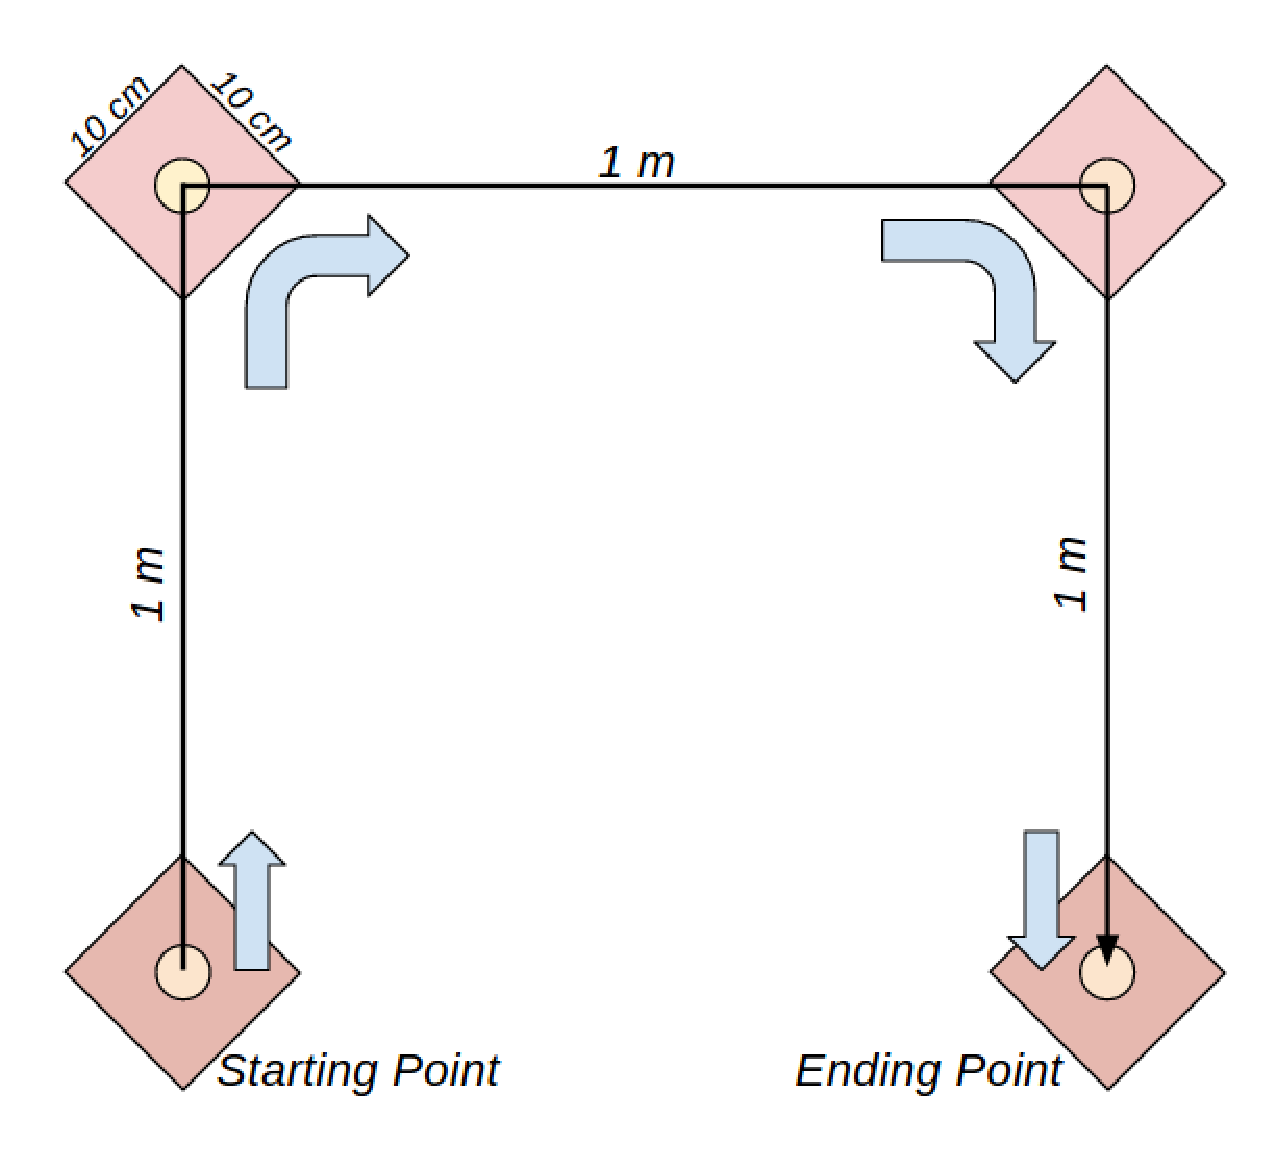
\includegraphics[width = 0.38\textwidth]{ExperimentTask}
\caption{Experiment Path}
\label{fig:ExperimentTask}
\end{figure} 

\subsubsection{Conditions}
Our experiments have two conditions: TD and KD. In TD, participants give only motion control instructions, while in KD, participants give both motion control instructions and the keyframe recording instruction.  We use a within-subject design to better control the differences between subjects.

\subsection{Experiment Protocol}
Each participant does two groups of teaching using TD and KD, respectively. The order of the two methods is counterbalanced. Each group involves 3 attempts. Each attempt consists of 2 phases, i.e., the teaching phase and the execution phase. 


In the teaching phase, participants are free to deploy any strategies based on the instruction set of the teaching method they are using, in order to improve the effectiveness of their teaching. In the execution phase, the participants are allowed to observe the robot's behavior. Participants are allowed to adjust their strategies between different attempts based on their observation of the execution phases. 

\subsection{Measures}  
The experiment results are evaluated in terms of a Teaching Effectiveness Index (TEX) and a Teaching Task Load Index (TLX). Subjective and objective measures are combined to achieve comprehensive evaluations. 

\subsubsection{Teaching Effectiveness Index} 
Three dependent variables are measured in the execution phase for each attempt, as listed below. 

\begin{itemize}
\item Trend ($T$, objective measure), i.e., whether or not the robot successfully reproduce the trend of the navigation path, as measured by a 3-level criteria:
\begin{itemize} 
\item Successful ($T = 2$) if the robot makes two right turns along the way and the angle errors are within 5 degrees; 
\item Not quite successful ($T = 1$) if the robot makes two right turns along the way but the angle errors are greater than 5 degrees but less than 60 degrees;
\item Unsuccessful ($T = 0$) if the robot behaves otherwise. 
\end{itemize} 

\item Accuracy ($A$, objective measure), i.e., whether or not the robot accurately follows the navigation path, as measured by a 3-level criteria: 
\begin{itemize}
\item Accurate ($A = 2$) if the robot follows the centerline of the navigation path with less than $\pm$10 cm error along the way; 
\item Not quite accurate ($A = 1$) if the robot is sometimes out of the $\pm$10 cm bound but always within $\pm$15 cm bound along the way; 
\item Inaccurate ($A = 0$) if the robot behaves otherwise. 
\end{itemize}

\item Human teacher evaluation ($E$, subjective measure), i.e., whether or not the human teacher considers the path reproduction as successful, as measured by a 3-level criteria: successful ($E = 2$), not quite successful ($E = 1$) or unsuccessful ($E = 0$).
\end{itemize} 

The teaching effectiveness of each demonstration method is evaluated by combining the three dependent variables of each attempt and averaging the evaluation results of the three attempts, as described by 
$$TEX = 0.4 \cdot avg(T[1:3]) + 0.2 \cdot avg(A[1:3]) + 0.4 \cdot avg(E[1:3]) $$ 

\subsubsection{Task Load Index}
We use the NASA Task Load Index (NASA TLX) to evaluate the human teacher's task load in the path teaching scenario. Each participant is asked to fill a NASA TLX evaluation form for each demonstration method. The evaluation form consists of six parts: Mental Demand (MD), Physical Demand (PD), Temporal Demand (TD), Performance (PF), Effort (EF) and Frustration (FR). We do not take TD and PF into the combined evaluation of TLX since we do not set time limits for the teaching task and we have already taken the teacher's subjective evaluation of the task performance into account in TEX. So the task load of each demonstration method is evaluated as 
$$TLX=avg([MD, PD, EF, FR]) $$

\begin{figure}
\centering
\includegraphics[width = 0.38\textwidth]{TEX}
\caption{Teaching Effectiveness Result}
\label{fig:TEX}
\end{figure} 

\begin{figure}
\centering
\includegraphics[width = 0.38\textwidth]{TLX}
\caption{NASA Task Load Result}
\label{fig:TLX}
\end{figure} 

\section{Results} 
We collected data from 10 participants and calculate TEX and TLX based on the experiment results. 

Figure~\ref{fig:TEX}. shows the result Teaching Effectiveness measurements from the experiments. KD get higher scores consider all three measurement aspects. Both TD and KD get high scores in aspect of Trend, which means the robot learnt correct direction according to the trajectory. However TD get much higher score in aspect of Accuracy. Only one teacher get partial success on TD learning on average which cause the single point in Accuracy column in Figure~\ref{fig:TEX}. The robot either doesn't move smoothly to the next target point or turns at the point that falls outside the 10cm range around the corner point. Only 2 partial success happens in all 60 times of learning. The robot either successfully moves along the designed trajectory or has large error at the beginning of the path. The large error happening at the very start point, usually along the first line segment, causes the position inaccuracy in the following movement consequently. 

The higher Accuracy scores also leads to higher scores of KD in terms of Teacher Evaluation of learnt trajectory. The accuracy aspects vector has very high correlation with Teacher Evaluation vector(Pearson correlation of 0.82), while the Trend vector has fairly low correlation towards Teacher Evaluation vector(Pearson correlation of 0.40). In other words, the participants focus more on the accuracy of learnt trajectory, regardless of the correct trend of robot movement.

Figure~\ref{fig:TLX}. shows the result NASA Task Load measurements from the experiments. TD get lower TLX. The differences between TD and KD in PD is fairly small because the instructors are only required to give verbal instructions to guide the robot. The differences scores on MD, EF and FR will discussed in the Discussion section.

Noticed that the range of user evaluation of NASA task load various a lot between teachers, we apply Wilcoxon signed rank test on our experiment result, which pair up the rankings from the same users.

\section{Discussion} 
In this section, we explain the observations from the experiments and further discuss the experimental results shown in the last section. 

\subsection{Limitations of the Robotic Platform}
As shown in Section 5, the simulation results show that, no matter which demonstration method is used, the learning algorithm can precisely reproduce the demonstrated navigation path. However, in the experiments based on Sphero, large deviation from the desired path is observed, especially in the case of TD. Such an inconsistency is caused  by the limited accuracy of Sphero's velocity control and self-localization. As is observed from the experiments, the actual moving direction of the robot can be up to 10 degrees away from the desired headings given by the velocity control signals, and the error of self-localization can be up to 15 cm.  


Apart from the noise of the robot sensors and the inaccurate nature of the navigation and localization system, other factors also contribute to the deviation that is observed during experiments. 


Firstly, the inertia of the robot causes undesirable displacement that is undetectable by the robot sensors. One common situation is that the robot keeps spinning for a short period of time when it suddenly stops on receiving a ``Stop'' instruction. The spinning causes up to 3 cm of displacement without being detected by the self-localization system. Another situation that is observed in our experiments is that a turn instruction is received when the robot is still moving and the angle of the turn has an error of up to 5 degrees due to the previous spinning state of the robot. 


Secondly, the robot's coordinate system is rotated by an angle of up to 5 degrees when a collision happens. Such a rotation causes inconvenience in the human teacher's demonstration (since the moving direction of the robot is no longer the same with what is expected), and also causes error in reproducing the navigation path since the frames that are recorded are not in terms of the rotated coordinate system.  


Finally, the unevenness of the friction caused by carpet patterns also contribute to the error in velocity control. Such unevenness gives different amount of friction in different directions, which results in different speed deviations in different directions, and thus an error of the robot's moving direction is caused. 

\subsection{TD Requires Less Task Load} 
TD casts less task load on teachers (P = 0.074 in Wilcoxon signed rank test) according to the result collected from the experiment.
 
The difference of LTX mainly comes from MD and FR as shown in Figure ~\ref{fig:TLX}. The mental demand of KD is because KD requires the teacher giving extra instruction when the robot approached the corner points, or the position that teacher feels is important. 
FR also contributes great portion towards LTX. This mainly because teachers forgot to keep certain frame on the corner and realized it before keep next frame. The teachers then tried to guide the robot move back to the last keyframe end position. This process causes frustrated feeling on teachers. 

Again, due to the limitation of the robot platform, both TD and KD require the teachers put effort the guide the robot. They usually find the latency between the give instructions and the robot response to the instruction, and then try to accommodate to this latency by giving the instructions when the robot approaching its next target point. This process requires extra effort of teachers. In future work, the language recognize process should be optimized to reduce the system setup limitation effect on the experiment result. 

\subsection{KD is More Effective} 
As shown in the result section, KD has better performance than TD in terms of effectiveness considering all trend, accuracy and teacher evaluation (P = 0.027 in Wilcoxon signed rank test ). 

The Figure ~\ref{fig:TEX}. shows that robot learnt trajectory from TD and KD get similar trend scores, but the learnt from KD has much better scores in accuracy. This could be due to as the system keep all the data sampled along TD, the position noise and error get accumulated along the time. This will not necessary affect the clustering results because the relative position between each sample position may remain accurate, but the recommendation given by the model may has error because the model gives target position in absolute value due to the limitation of robot platform we discussed in previous section.

Another possible reason that cause the accuracy difference is the TD may not collect enough data at the corner points to make it a stand-alone cluster. In simulation, the turtles node stay in the corner for a period of time waiting for turning into its target direction. In the experiment setup, in contrast, teacher usually let the robot stay at the corner for fairly short of time, or even given turning instruction in advance to the robot approaching the corner. This will cause the GMM clustering the corner into its adjacent line segment. The model will then give the robot recommendation directly goes to the mean of next line segment instead of going to the corner first. The KD have no issue with sample data distribution because almost all the users successfully keep the corner points as one of key points.

\subsection{Teaching Strategies}  
We found from our observations that different human teachers tend to use different teaching strategies, and they usually deliberately adjust their strategies between demonstrations attempting to improve the robot's performance.

\subsubsection{TD Strategies}
One commonly observed strategy difference in TD is that while most human teachers make the robot stop before giving a turn instruction, a few directly give turn instructions while the robot is still moving. Some teachers turn the robot using different strategies in different demonstrations, attempting to improve the teaching effectiveness by trying different strategies. Some even combine the two strategies in one demonstration. 


from the data collected from those participants who use both the stop-and-turn and the turn-without-stopping strategies, we observe a slight enhancement of teaching effectiveness by using the turn-without-stopping strategy. As is stated in the first part of this section, sudden stops in the movement of the robot causes undesirable displacement which the sensors are not able to detect. Therefore, the turn-without-stopping strategy improves the teaching effectiveness by reducing the navigation errors of the robotic platform. 

\subsubsection{KD Strategies}
Three strategy differences are observed in KD during the experiments. Firstly, most teachers make the robot stop before giving a ``Keep this frame'' instruction, while a few teachers give ``Keep this frame'' instructions while the robot is moving. Secondly, teachers use different granularities of frames, i.e., different frequencies of using ``Keep this frame'', along the navigation path. Some teachers attempt to increase the frame granularity to improve the teaching effectiveness. Thirdly, some teachers try following the path as accurately as possible during their demonstrations, while others, knowing that only the keyframes will be remembered by the robot, only try keeping the keyframes accurately, not constrained by the paths the robot takes to reach those keyframe positions. 


Our experiments show that the stop-and-keep-this-frame strategy helps the teachers to keep the desired keyframes accurately. Most teachers choose the turning point of the path as keyframes, in which case it is hard to get the accurate keyframes if the ``Keep this frame'' instruction is given without first putting the robot to a stop. 


One participant tries different keyframe granularities in his demonstrations. Apart from the turning point, he adds some middle points of straight-line parts of the path in one of his demonstration. The result shows that, by adding extra keyframes, even though the robot still reproduces the trend of the path correctly, the accuracy is undermined. Such a result can be explained by extra self-localization errors caused by additional sub-destinations. However, it is hard to tell whether this is a common trend since only one comparison is done. 


Several participants simply guide the robot to reach the turning points one after another. Sometimes the between-keyframe paths can be far deviated from the desired path. Such deviation does not make an observable difference in the effectiveness of teaching since the robot does not remember anything about the between-keyframe paths. However, these teachers' subjective evaluation of mental demand is higher due to the extra effort taken to make the keyframes as accurate as possible. 

\subsubsection{Path Adjustment}
Another strategy that is used by teachers during our experiments is path adjustment, whereby the teacher adjusts the shape of the path they demonstrate to the robot to compensate the navigation error that is observed in previous demonstration attempts. Such a strategy can be used to compensate errors with predictable directions. For example, if it is observed that the robot skews its path toward the right side of the desired path in the past two demonstration attempts, the teacher can adjust the path to the left when she/he gives the third demonstration. In our experiments, only one participant deliberately uses such path adjustment strategy, which gives the best learning effectiveness of TD among all TD attempts of all participants.  

\section{Conclusions} 
In this paper, demonstration methods in LfD are explored in the path teaching scenario. Specifically, two demonstration methods, TD and KD, are compared in two aspects, i.e., the demonstration methods' effectiveness and the human teacher's task load. Algorithms are implemented based on Sphero SPRK, and experiments designed and conducted to do the comparison using both subjective and objective measures. 


Due to the limitations of the robotic platform, the robot's learning performance is undermined by the inaccuracy of velocity control and self-localization. Although the path reproduction is accurate in simulations no matter which demonstration method is used, it is not as accurate in the experiments using Sphero, where the difference in effectiveness of different demonstration methods shows up. Our experimental results show that, in general, while TD requires less task load from the human teacher, KD is more effective in terms of the robot's performance of reproducing the demonstrated navigation path. 


We also found from our observations that different human teachers tend to use different teaching strategies, and they usually deliberately adjust their strategies between demonstrations attempting to improve the robot's performance. And our experiments show that human teacher's strategies have a considerable effect on the effectiveness of teaching. 

\section{Acknowledgement} 
We want to acknowledge Prof. Andrea L. Thomaz for providing the robotic platform and giving valuable advices during different phases of this research. We also acknowledge those students of The University of Texas at Austin who have participated in our experiments. 

\section{References}
\noindent {[}1{]} Akgun, B., Cakmak, M., Jiang, K., \& Thomaz, A. L. (2012). Keyframe-based learning from demonstration. International Journal of Social Robotics, 4(4), 343-355.\\
{[}2{]} Akgun, B., Cakmak, M., Yoo, J. W., \& Thomaz, A. L. (2012, March). Trajectories and keyframes for kinesthetic teaching: A human-robot interaction perspective. In Proceedings of the seventh annual ACM/IEEE international conference on Human-Robot Interaction (pp. 391-398). ACM.\\
{[}3{]} Argall, B. D., Chernova, S., Veloso, M., \& Browning, B. (2009). A survey of robot learning from demonstration. Robotics and autonomous systems, 57(5), 469-483.\\
{[}4{]} Khansari-Zadeh, S. M., \& Billard, A. (2011). Learning stable nonlinear dynamical systems with gaussian mixture models. IEEE Transactions on Robotics, 27(5), 943-957.\\
{[}5{]} Pastor, P., Hoffmann, H., Asfour, T., \& Schaal, S. (2009, May). Learning and generalization of motor skills by learning from demonstration. In Robotics and Automation, 2009. ICRA'09. IEEE International Conference on (pp. 763-768). IEEE.\\
{[}6{]} F. Bashir, A. Khokhar and D. Schonfeld, Automatic Object Trajectory-Based Motion Recognition Using Gaussian Mixture Models, 2005 IEEE International Conference on Multimedia and Expo, Amsterdam, 2005, pp. 1532-1535.\\
{[}7{]} F. I. Bashir, A. A. Khokhar and D. Schonfeld, Object Trajectory-Based Activity Classification and Recognition Using Hidden Markov Models, in IEEE Transactions on Image Processing, vol. 16, no. 7, pp. 1912-1919, July 2007.\\
{[}8{]} A. Vakanski, I. Mantegh, A. Irish and F. Janabi-Sharifi, Trajectory Learning for Robot Programming by Demonstration Using Hidden Markov Model and Dynamic Time Warping, in IEEE Transactions on Systems, Man, and Cybernetics, Part B (Cybernetics), vol. 42, no. 4, pp. 1039-1052, Aug. 2012.\\

%\section{The {\secit Body} of The Paper}
%Typically, the body of a paper is organized
%into a hierarchical structure, with numbered or unnumbered
%headings for sections, subsections, sub-subsections, and even
%smaller sections.  The command \texttt{{\char'134}section} that
%precedes this paragraph is part of such a
%hierarchy.\footnote{This is the second footnote.  It
%starts a series of three footnotes that add nothing
%informational, but just give an idea of how footnotes work
%and look. It is a wordy one, just so you see
%how a longish one plays out.} \LaTeX\ handles the numbering
%and placement of these headings for you, when you use
%the appropriate heading commands around the titles
%of the headings.  If you want a sub-subsection or
%smaller part to be unnumbered in your output, simply append an
%asterisk to the command name.  Examples of both
%numbered and unnumbered headings will appear throughout the
%balance of this sample document.
%
%Because the entire article is contained in
%the \textbf{document} environment, you can indicate the
%start of a new paragraph with a blank line in your
%input file; that is why this sentence forms a separate paragraph.
%
%\subsection{Type Changes and {\subsecit Special} Characters}
%We have already seen several typeface changes in this sample.  You
%can indicate italicized words or phrases in your text with
%the command \texttt{{\char'134}textit}; emboldening with the
%command \texttt{{\char'134}textbf}
%and typewriter-style (for instance, for computer code) with
%\texttt{{\char'134}texttt}.  But remember, you do not
%have to indicate typestyle changes when such changes are
%part of the \textit{structural} elements of your
%article; for instance, the heading of this subsection will
%be in a sans serif\footnote{A third footnote, here.
%Let's make this a rather short one to
%see how it looks.} typeface, but that is handled by the
%document class file. Take care with the use
%of\footnote{A fourth, and last, footnote.}
%the curly braces in typeface changes; they mark
%the beginning and end of
%the text that is to be in the different typeface.
%
%You can use whatever symbols, accented characters, or
%non-English characters you need anywhere in your document;
%you can find a complete list of what is
%available in the \textit{\LaTeX\
%User's Guide}\cite{Lamport:LaTeX}.
%
%\subsection{Math Equations}
%You may want to display math equations in three distinct styles:
%inline, numbered or non-numbered display.  Each of
%the three are discussed in the next sections.
%
%\subsubsection{Inline (In-text) Equations}
%A formula that appears in the running text is called an
%inline or in-text formula.  It is produced by the
%\textbf{math} environment, which can be
%invoked with the usual \texttt{{\char'134}begin. . .{\char'134}end}
%construction or with the short form \texttt{\$. . .\$}. You
%can use any of the symbols and structures,
%from $\alpha$ to $\omega$, available in
%\LaTeX\cite{Lamport:LaTeX}; this section will simply show a
%few examples of in-text equations in context. Notice how
%this equation: \begin{math}\lim_{n\rightarrow \infty}x=0\end{math},
%set here in in-line math style, looks slightly different when
%set in display style.  (See next section).
%
%\subsubsection{Display Equations}
%A numbered display equation -- one set off by vertical space
%from the text and centered horizontally -- is produced
%by the \textbf{equation} environment. An unnumbered display
%equation is produced by the \textbf{displaymath} environment.
%
%Again, in either environment, you can use any of the symbols
%and structures available in \LaTeX; this section will just
%give a couple of examples of display equations in context.
%First, consider the equation, shown as an inline equation above:
%\begin{equation}\lim_{n\rightarrow \infty}x=0\end{equation}
%Notice how it is formatted somewhat differently in
%the \textbf{displaymath}
%environment.  Now, we'll enter an unnumbered equation:
%\begin{displaymath}\sum_{i=0}^{\infty} x + 1\end{displaymath}
%and follow it with another numbered equation:
%\begin{equation}\sum_{i=0}^{\infty}x_i=\int_{0}^{\pi+2} f\end{equation}
%just to demonstrate \LaTeX's able handling of numbering.
%
%\subsection{Citations}
%Citations to articles \cite{bowman:reasoning,
%clark:pct, braams:babel, herlihy:methodology},
%conference proceedings \cite{clark:pct} or
%books \cite{salas:calculus, Lamport:LaTeX} listed
%in the Bibliography section of your
%article will occur throughout the text of your article.
%You should use BibTeX to automatically produce this bibliography;
%you simply need to insert one of several citation commands with
%a key of the item cited in the proper location in
%the \texttt{.tex} file \cite{Lamport:LaTeX}.
%The key is a short reference you invent to uniquely
%identify each work; in this sample document, the key is
%the first author's surname and a
%word from the title.  This identifying key is included
%with each item in the \texttt{.bib} file for your article.
%
%The details of the construction of the \texttt{.bib} file
%are beyond the scope of this sample document, but more
%information can be found in the \textit{Author's Guide},
%and exhaustive details in the \textit{\LaTeX\ User's
%Guide}\cite{Lamport:LaTeX}.
%
%This article shows only the plainest form
%of the citation command, using \texttt{{\char'134}cite}.
%This is what is stipulated in the SIGS style specifications.
%No other citation format is endorsed or supported.
%
%\subsection{Tables}
%Because tables cannot be split across pages, the best
%placement for them is typically the top of the page
%nearest their initial cite.  To
%ensure this proper ``floating'' placement of tables, use the
%environment \textbf{table} to enclose the table's contents and
%the table caption.  The contents of the table itself must go
%in the \textbf{tabular} environment, to
%be aligned properly in rows and columns, with the desired
%horizontal and vertical rules.  Again, detailed instructions
%on \textbf{tabular} material
%is found in the \textit{\LaTeX\ User's Guide}.
%
%Immediately following this sentence is the point at which
%Table 1 is included in the input file; compare the
%placement of the table here with the table in the printed
%dvi output of this document.
%
%\begin{table}
%\centering
%\caption{Frequency of Special Characters}
%\begin{tabular}{|c|c|l|} \hline
%Non-English or Math&Frequency&Comments\\ \hline
%\O & 1 in 1,000& For Swedish names\\ \hline
%$\pi$ & 1 in 5& Common in math\\ \hline
%\$ & 4 in 5 & Used in business\\ \hline
%$\Psi^2_1$ & 1 in 40,000& Unexplained usage\\
%\hline\end{tabular}
%\end{table}
%
%To set a wider table, which takes up the whole width of
%the page's live area, use the environment
%\textbf{table*} to enclose the table's contents and
%the table caption.  As with a single-column table, this wide
%table will ``float" to a location deemed more desirable.
%Immediately following this sentence is the point at which
%Table 2 is included in the input file; again, it is
%instructive to compare the placement of the
%table here with the table in the printed dvi
%output of this document.
%
%
%\begin{table*}
%\centering
%\caption{Some Typical Commands}
%\begin{tabular}{|c|c|l|} \hline
%Command&A Number&Comments\\ \hline
%\texttt{{\char'134}alignauthor} & 100& Author alignment\\ \hline
%\texttt{{\char'134}numberofauthors}& 200& Author enumeration\\ \hline
%\texttt{{\char'134}table}& 300 & For tables\\ \hline
%\texttt{{\char'134}table*}& 400& For wider tables\\ \hline\end{tabular}
%\end{table*}
%% end the environment with {table*}, NOTE not {table}!
%
%\subsection{Figures}
%Like tables, figures cannot be split across pages; the
%best placement for them
%is typically the top or the bottom of the page nearest
%their initial cite.  To ensure this proper ``floating'' placement
%of figures, use the environment
%\textbf{figure} to enclose the figure and its caption.
%
%This sample document contains examples of \textbf{.eps} files to be
%displayable with \LaTeX.  If you work with pdf\LaTeX, use files in the
%\textbf{.pdf} format.  Note that most modern \TeX\ system will convert
%\textbf{.eps} to \textbf{.pdf} for you on the fly.  More details on
%each of these is found in the \textit{Author's Guide}.
%
%\begin{figure}
%\centering
%\includegraphics{fly}
%\caption{A sample black and white graphic.}
%\end{figure}
%
%\begin{figure}
%\centering
%\includegraphics[height=1in, width=1in]{fly}
%\caption{A sample black and white graphic
%that has been resized with the \texttt{includegraphics} command.}
%\end{figure}
%
%
%As was the case with tables, you may want a figure
%that spans two columns.  To do this, and still to
%ensure proper ``floating'' placement of tables, use the environment
%\textbf{figure*} to enclose the figure and its caption.
%and don't forget to end the environment with
%{figure*}, not {figure}!
%
%\begin{figure*}
%\centering
%\includegraphics{flies}
%\caption{A sample black and white graphic
%that needs to span two columns of text.}
%\end{figure*}
%
%
%\begin{figure}
%\centering
%\includegraphics[height=1in, width=1in]{rosette}
%\caption{A sample black and white graphic that has
%been resized with the \texttt{includegraphics} command.}
%\vskip -6pt
%\end{figure}
%
%\subsection{Theorem-like Constructs}
%Other common constructs that may occur in your article are
%the forms for logical constructs like theorems, axioms,
%corollaries and proofs.  There are
%two forms, one produced by the
%command \texttt{{\char'134}newtheorem} and the
%other by the command \texttt{{\char'134}newdef}; perhaps
%the clearest and easiest way to distinguish them is
%to compare the two in the output of this sample document:
%
%This uses the \textbf{theorem} environment, created by
%the\linebreak\texttt{{\char'134}newtheorem} command:
%\newtheorem{theorem}{Theorem}
%\begin{theorem}
%Let $f$ be continuous on $[a,b]$.  If $G$ is
%an antiderivative for $f$ on $[a,b]$, then
%\begin{displaymath}\int^b_af(t)dt = G(b) - G(a).\end{displaymath}
%\end{theorem}
%
%The other uses the \textbf{definition} environment, created
%by the \texttt{{\char'134}newdef} command:
%\newdef{definition}{Definition}
%\begin{definition}
%If $z$ is irrational, then by $e^z$ we mean the
%unique number which has
%logarithm $z$: \begin{displaymath}{\log e^z = z}\end{displaymath}
%\end{definition}
%
%Two lists of constructs that use one of these
%forms is given in the
%\textit{Author's  Guidelines}.
% 
%There is one other similar construct environment, which is
%already set up
%for you; i.e. you must \textit{not} use
%a \texttt{{\char'134}newdef} command to
%create it: the \textbf{proof} environment.  Here
%is a example of its use:
%\begin{proof}
%Suppose on the contrary there exists a real number $L$ such that
%\begin{displaymath}
%\lim_{x\rightarrow\infty} \frac{f(x)}{g(x)} = L.
%\end{displaymath}
%Then
%\begin{displaymath}
%l=\lim_{x\rightarrow c} f(x)
%= \lim_{x\rightarrow c}
%\left[ g{x} \cdot \frac{f(x)}{g(x)} \right ]
%= \lim_{x\rightarrow c} g(x) \cdot \lim_{x\rightarrow c}
%\frac{f(x)}{g(x)} = 0\cdot L = 0,
%\end{displaymath}
%which contradicts our assumption that $l\neq 0$.
%\end{proof}
%
%Complete rules about using these environments and using the
%two different creation commands are in the
%\textit{Author's Guide}; please consult it for more
%detailed instructions.  If you need to use another construct,
%not listed therein, which you want to have the same
%formatting as the Theorem
%or the Definition\cite{salas:calculus} shown above,
%use the \texttt{{\char'134}newtheorem} or the
%\texttt{{\char'134}newdef} command,
%respectively, to create it.
%
%\subsection*{A {\secit Caveat} for the \TeX\ Expert}
%Because you have just been given permission to
%use the \texttt{{\char'134}newdef} command to create a
%new form, you might think you can
%use \TeX's \texttt{{\char'134}def} to create a
%new command: \textit{Please refrain from doing this!}
%Remember that your \LaTeX\ source code is primarily intended
%to create camera-ready copy, but may be converted
%to other forms -- e.g. HTML. If you inadvertently omit
%some or all of the \texttt{{\char'134}def}s recompilation will
%be, to say the least, problematic.
%
%\section{Conclusions}
%This paragraph will end the body of this sample document.
%Remember that you might still have Acknowledgments or
%Appendices; brief samples of these
%follow.  There is still the Bibliography to deal with; and
%we will make a disclaimer about that here: with the exception
%of the reference to the \LaTeX\ book, the citations in
%this paper are to articles which have nothing to
%do with the present subject and are used as
%examples only.
%%\end{document}  % This is where a 'short' article might terminate
%
%%ACKNOWLEDGMENTS are optional
%\section{Acknowledgments}
%This section is optional; it is a location for you
%to acknowledge grants, funding, editing assistance and
%what have you.  In the present case, for example, the
%authors would like to thank Gerald Murray of ACM for
%his help in codifying this \textit{Author's Guide}
%and the \textbf{.cls} and \textbf{.tex} files that it describes.
%
%%
%% The following two commands are all you need in the
%% initial runs of your .tex file to
%% produce the bibliography for the citations in your paper.
%\bibliographystyle{abbrv}
%\bibliography{sigproc}  % sigproc.bib is the name of the Bibliography in this case
%% You must have a proper ".bib" file
%%  and remember to run:
%% latex bibtex latex latex
%% to resolve all references
%%
%% ACM needs 'a single self-contained file'!
%%
%%APPENDICES are optional
%%\balancecolumns
%\appendix
%%Appendix A
%\section{Headings in Appendices}
%The rules about hierarchical headings discussed above for
%the body of the article are different in the appendices.
%In the \textbf{appendix} environment, the command
%\textbf{section} is used to
%indicate the start of each Appendix, with alphabetic order
%designation (i.e. the first is A, the second B, etc.) and
%a title (if you include one).  So, if you need
%hierarchical structure
%\textit{within} an Appendix, start with \textbf{subsection} as the
%highest level. Here is an outline of the body of this
%document in Appendix-appropriate form:
%\subsection{Introduction}
%\subsection{The Body of the Paper}
%\subsubsection{Type Changes and  Special Characters}
%\subsubsection{Math Equations}
%\paragraph{Inline (In-text) Equations}
%\paragraph{Display Equations}
%\subsubsection{Citations}
%\subsubsection{Tables}
%\subsubsection{Figures}
%\subsubsection{Theorem-like Constructs}
%\subsubsection*{A Caveat for the \TeX\ Expert}
%\subsection{Conclusions}
%\subsection{Acknowledgments}
%\subsection{Additional Authors}
%This section is inserted by \LaTeX; you do not insert it.
%You just add the names and information in the
%\texttt{{\char'134}additionalauthors} command at the start
%of the document.
%\subsection{References}
%Generated by bibtex from your ~.bib file.  Run latex,
%then bibtex, then latex twice (to resolve references)
%to create the ~.bbl file.  Insert that ~.bbl file into
%the .tex source file and comment out
%the command \texttt{{\char'134}thebibliography}.
%% This next section command marks the start of
%% Appendix B, and does not continue the present hierarchy
%\section{More Help for the Hardy}
%The sig-alternate.cls file itself is chock-full of succinct
%and helpful comments.  If you consider yourself a moderately
%experienced to expert user of \LaTeX, you may find reading
%it useful but please remember not to change it.
%%\balancecolumns % GM June 2007
%% That's all folks!
\]
\end{document}